
\documentclass{article}
% \usepackage{amsmath}
\usepackage{geometry}
\usepackage{graphicx} % Required for inserting images
\usepackage{listings}
\usepackage{color}
\usepackage{verbatim} 
\usepackage{fancyvrb}
\usepackage{fvextra}

\graphicspath{ {./gtkwave/} }

\definecolor{dkgreen}{rgb}{0,0.6,0}
\definecolor{gray}{rgb}{0.5,0.5,0.5}
\definecolor{mauve}{rgb}{0.58,0,0.82}

\lstset{frame=tb,
  language=Verilog,
  aboveskip=3mm,
  belowskip=3mm,
  showstringspaces=false,
  columns=flexible,
  basicstyle={\small\ttfamily},
  numbers=none,
  numberstyle=\tiny\color{gray},
  keywordstyle=\color{blue},
  commentstyle=\color{dkgreen},
  stringstyle=\color{mauve},
  breaklines=true,
  breakatwhitespace=true,
  tabsize=3
}

\title{Digital Design Lab Report}
\author{Xiaokun Du}
\date{February 2023}

\begin{document}

% Creates a title based on the \title, \author, and \date provided
\maketitle


\section{Arithmetic logic unit (ALU)}

Write, as a SystemVerilog module with the name alu, a behavioural description of an arithmetic logic unit. \\
The data inputs, SrcA and SrcB, and the data output, ALUResult, are 8-bit vectors. The ALUControl input is a 2-bit vector. \\
The 1-bit output flag Zero = 1 if ALUResult == 0, else Zero = 0. The ALU carries out bitwise logical operations, and addition and subtraction operations, as specified in the table below.
\subsection{Module Code}
\begin{lstlisting}
module alu(input logic [7:0] SrcA,
            input logic [7:0] SrcB,
            input logic [1:0] ALUControl,
            output logic [7:0] ALUResult,
            output logic Zero);
always_comb
case (ALUControl)
2'b00 : ALUResult = SrcA & SrcB;
2'b01 : ALUResult = SrcA | SrcB;
2'b10 : ALUResult = SrcA + SrcB;
2'b11 : ALUResult = SrcA - SrcB;
default : ALUResult = 8'bx;
endcase

assign Zero = (ALUResult == 8'b0);
endmodule
\end{lstlisting}

\subsection{Testbench Code}
\begin{lstlisting}
`timescale 1ns/1ps 
`include "alu.sv"

module alu_tb;
logic [7:0] t_SrcA, t_SrcB;
logic [1:0] t_ALUControl;
logic [7:0] t_ALUResult;
logic t_Zero;

alu uut (t_SrcA, t_SrcB, t_ALUControl, t_ALUResult, t_Zero);

initial begin
    $dumpfile("alu_tb.vcd"); 
    $dumpvars(0, alu_tb);
    // Stimulus generator
    t_SrcA = 8'h05; t_SrcB = 8'h0A;
    t_ALUControl = 2'b00; #20;
    t_ALUControl = 2'b01; #20;
    t_ALUControl = 2'b10; #20;
    t_ALUControl = 2'b11; #20;
end

initial begin // Response monitor
    $monitor ("t_ALUControl = %b t_SrcA = %h t_SrcB = %h t_ALUResult = %b t_Zero = %d",t_ALUControl, t_SrcA, t_SrcB, t_ALUResult, t_Zero);
end
endmodule

\end{lstlisting}

\subsection{Simulations}
The simulation result using Icarus Verilog is as following:
\begin{Verbatim}
VCD info: dumpfile alu_tb.vcd opened for output.
t_ALUControl = 00 t_SrcA = 05 t_SrcB = 0a t_ALUResult = 00000000 t_Zero = 1
t_ALUControl = 01 t_SrcA = 05 t_SrcB = 0a t_ALUResult = 00001111 t_Zero = 0
t_ALUControl = 10 t_SrcA = 05 t_SrcB = 0a t_ALUResult = 00001111 t_Zero = 0
t_ALUControl = 11 t_SrcA = 05 t_SrcB = 0a t_ALUResult = 11111011 t_Zero = 0
\end{Verbatim}
The simulation results using GTKWave is as following:\vspace{5pt}\\
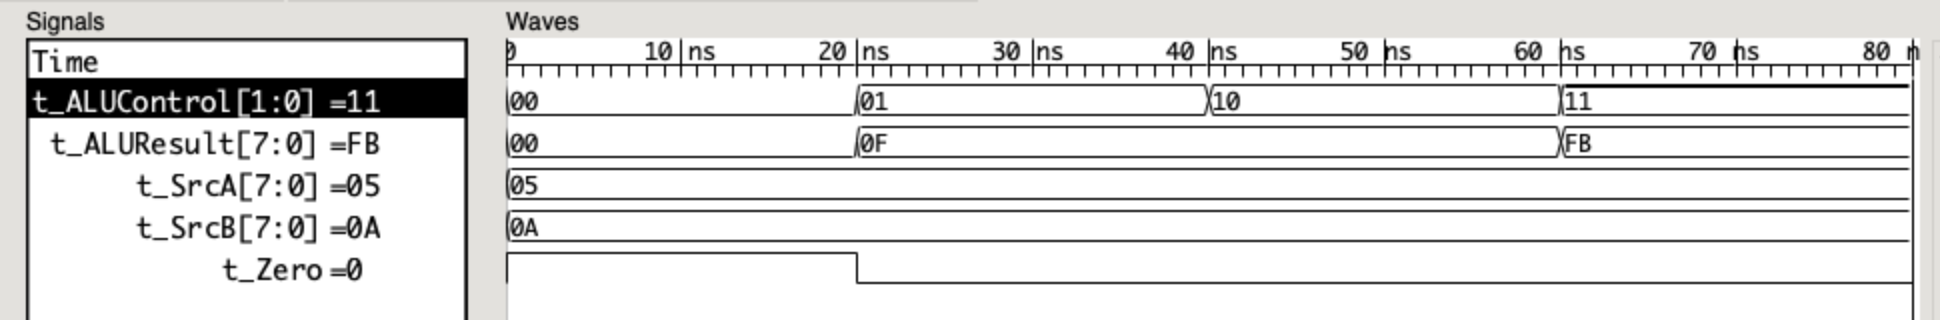
\includegraphics[width=\textwidth]{alu.png}

\newpage
\section{Register File}
The register file has sixteen 8-bit registers. The register with address 0 always contains the value 0. The other 15 registers can have values written into them through the WD3 port.\\
The contents of any two of the registers (with addresses specifiedby the 4-bit inputs RA1 and RA) are continuously output as RD1 and RD2. On the positive edge of the clock, if write\_enable is asserted, and A3 > 0, the input ALUResult is written into the register at address A3 through the WD3 port. The module includes an output port cpu\_out, which continuously outputs the contents of the register at address 15. This will form the main external output of the microprocessor.
\subsection{Module Code}
\begin{lstlisting}
    module reg_file(input logic [3:0] RA1, RA2, WA, 
                            input logic [7:0] ALUResult,
                            input logic clk, write_enable,
                            output logic [7:0] RD1, RD2, cpu_out); 
    logic [7:0] rf [0:15];
    logic [3:0] zero;

    assign RD1 = rf[RA1]; 
    assign RD2 = rf[RA2]; 
    assign cpu_out = rf[15];

    always_ff @(posedge clk) 
    if (write_enable && WA > 0) 
        rf[WA] = ALUResult;

    endmodule
\end{lstlisting}
\subsection{Testbench Code}
\begin{lstlisting}
    `timescale 1ps/1ps 
    `include "reg_file.sv"
    
    module reg_file_tb;
    logic [3:0] RA1, RA2, WA;
    logic clk, write_enable;
    logic [7:0] ALUResult, RD1, RD2, cpu_out;
    reg_file dut (RA1, RA2, WA, ALUResult, clk, write_enable, RD1, RD2, cpu_out);
    
    initial begin // Generate clock signal with 20 ns period
        clk = 0;
        forever #10 clk = ~clk;
    end
    
    initial begin // Apply stimulus 
        $dumpfile("reg_file_tb.vcd");
        $dumpvars(0, reg_file_tb);
        RA1 = 1; RA2 = 2; WA = 0; ALUResult = 5; write_enable = 0; 
        #15 write_enable = 1;
        #20 WA = 1; ALUResult = 7;
        #20 WA = 5; ALUResult = 13;
        #20 write_enable = 0;
        #10 RA2 = 5;
        #10;
        #10 WA = 15; write_enable = 1;
        #10 ALUResult = 15;
        #30;
        $finish; // This system tasks ends the simulation 
    end
    
    initial begin // Response monitor
      $monitor ("t = %3d, t_RA1 = %d t_RA2 = %d t_WA = %d ALUResult = %d t_clk = %d t_write_enable = %d t_RD1 = %d t_RD2 = %d t_cpu_out = %d",
                $time, RA1, RA2, WA, ALUResult, clk,  write_enable, RD1, RD2, cpu_out);
    end
    endmodule
\end{lstlisting}

\subsection{Simulations}
The simulation results using Icarus Verilog is as below:
\begin{Verbatim}[fontsize = \scriptsize]
t =   0, RA1 =  1 RA2 =  2 WA =  0 ALUResult =   5 clk = 0 write_enable = 0 RD1 =   x RD2 =   x cpu_out =   x
t =  10, RA1 =  1 RA2 =  2 WA =  0 ALUResult =   5 clk = 1 write_enable = 0 RD1 =   x RD2 =   x cpu_out =   x
t =  15, RA1 =  1 RA2 =  2 WA =  0 ALUResult =   5 clk = 1 write_enable = 1 RD1 =   x RD2 =   x cpu_out =   x
t =  20, RA1 =  1 RA2 =  2 WA =  0 ALUResult =   5 clk = 0 write_enable = 1 RD1 =   x RD2 =   x cpu_out =   x
t =  30, RA1 =  1 RA2 =  2 WA =  0 ALUResult =   5 clk = 1 write_enable = 1 RD1 =   x RD2 =   x cpu_out =   x
t =  35, RA1 =  1 RA2 =  2 WA =  1 ALUResult =   7 clk = 1 write_enable = 1 RD1 =   x RD2 =   x cpu_out =   x
t =  40, RA1 =  1 RA2 =  2 WA =  1 ALUResult =   7 clk = 0 write_enable = 1 RD1 =   x RD2 =   x cpu_out =   x
t =  50, RA1 =  1 RA2 =  2 WA =  1 ALUResult =   7 clk = 1 write_enable = 1 RD1 =   7 RD2 =   x cpu_out =   x
t =  55, RA1 =  1 RA2 =  2 WA =  5 ALUResult =  13 clk = 1 write_enable = 1 RD1 =   7 RD2 =   x cpu_out =   x
t =  60, RA1 =  1 RA2 =  2 WA =  5 ALUResult =  13 clk = 0 write_enable = 1 RD1 =   7 RD2 =   x cpu_out =   x
t =  70, RA1 =  1 RA2 =  2 WA =  5 ALUResult =  13 clk = 1 write_enable = 1 RD1 =   7 RD2 =   x cpu_out =   x
t =  75, RA1 =  1 RA2 =  2 WA =  5 ALUResult =  13 clk = 1 write_enable = 0 RD1 =   7 RD2 =   x cpu_out =   x
t =  80, RA1 =  1 RA2 =  2 WA =  5 ALUResult =  13 clk = 0 write_enable = 0 RD1 =   7 RD2 =   x cpu_out =   x
t =  85, RA1 =  1 RA2 =  5 WA =  5 ALUResult =  13 clk = 0 write_enable = 0 RD1 =   7 RD2 =  13 cpu_out =   x
t =  90, RA1 =  1 RA2 =  5 WA =  5 ALUResult =  13 clk = 1 write_enable = 0 RD1 =   7 RD2 =  13 cpu_out =   x
t = 100, RA1 =  1 RA2 =  5 WA =  5 ALUResult =  13 clk = 0 write_enable = 0 RD1 =   7 RD2 =  13 cpu_out =   x
t = 105, RA1 =  1 RA2 =  5 WA = 15 ALUResult =  13 clk = 0 write_enable = 1 RD1 =   7 RD2 =  13 cpu_out =   x
t = 110, RA1 =  1 RA2 =  5 WA = 15 ALUResult =  13 clk = 1 write_enable = 1 RD1 =   7 RD2 =  13 cpu_out =  13
t = 115, RA1 =  1 RA2 =  5 WA = 15 ALUResult =  15 clk = 1 write_enable = 1 RD1 =   7 RD2 =  13 cpu_out =  13
t = 120, RA1 =  1 RA2 =  5 WA = 15 ALUResult =  15 clk = 0 write_enable = 1 RD1 =   7 RD2 =  13 cpu_out =  13
t = 130, RA1 =  1 RA2 =  5 WA = 15 ALUResult =  15 clk = 1 write_enable = 1 RD1 =   7 RD2 =  13 cpu_out =  15
t = 140, RA1 =  1 RA2 =  5 WA = 15 ALUResult =  15 clk = 0 write_enable = 1 RD1 =   7 RD2 =  13 cpu_out =  15 
\end{Verbatim}
The simulation results using GTKWave is as following:\vspace{5pt}\\
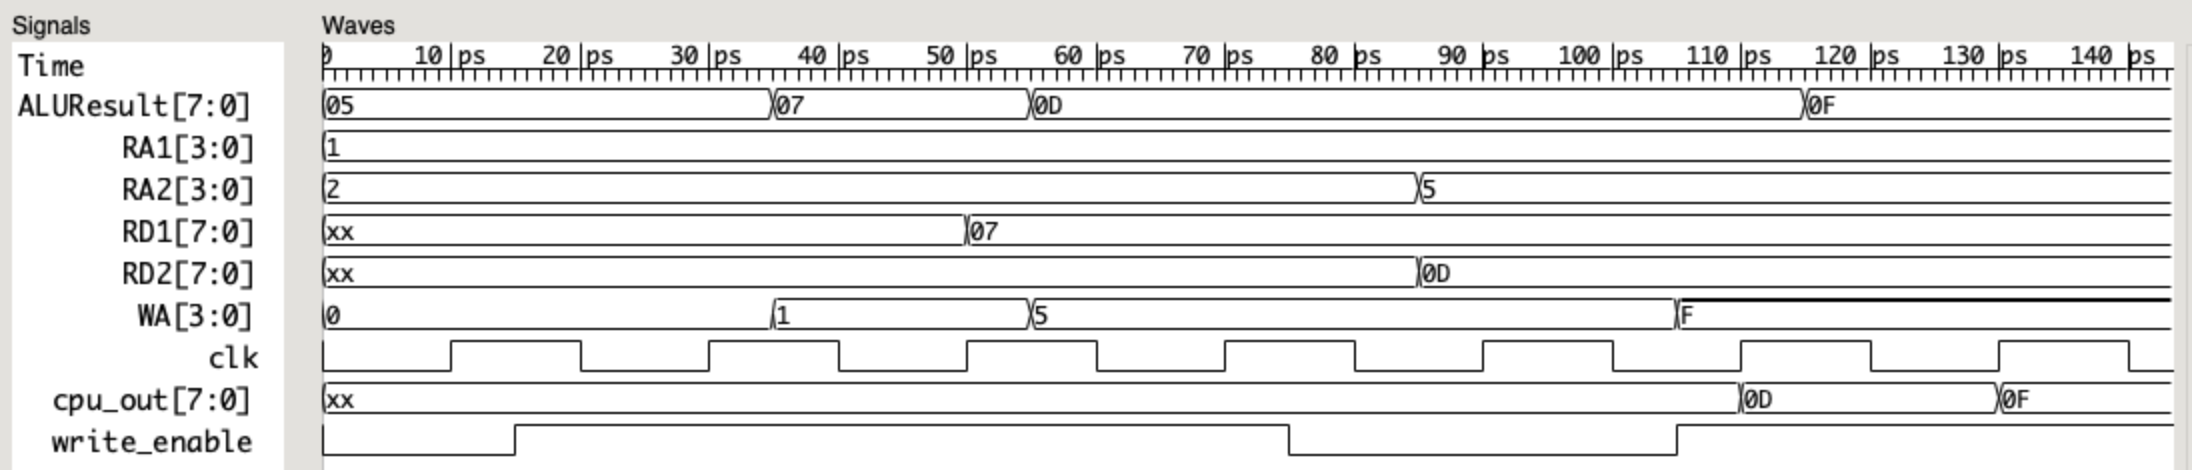
\includegraphics[width=\textwidth]{reg_file.png}

\newpage
\section{Combining the ALU and register file}
Write a SystemVerilog module with the name reg\_file\_alu, implementing the combined ALU and register file as shown above.
Include a 2-to-1 multiplexer, which selects either the RD2 output from the register file, or an external input (immediate) to be input to the ALU input port SrcB.

\subsection{Module Code}
\begin{lstlisting}
`include "reg_file.sv", "alu.sv"

module reg_file_alu(input logic [3:0] RA1, RA2, WA,
                    input logic [7:0] immediate,
                    input logic [1:0] ALUControl,
                    input logic write_enable, ALUSrc, CLK,
                    output logic [7:0] ALUResult, cpu_out,
                    output logic Zero);
logic A, B, B0, C;

reg_file(RA1, RA2, WA, C, CLK, write_enable, A, B0, cpu_out);
alu(A, B, ALUControl, ALUResult, Zero);
// 2 to 1 multiplexer
assign B = (ALUSrc) ? immediate : RD2;
endmodule

\end{lstlisting}


\end{document}
